\documentclass[11pt,a4paper,titlepage, ngerman]{article}

\usepackage[utf8]{inputenc}	
\usepackage[T1]{fontenc}	
\usepackage{ngerman}			
\usepackage{lmodern}			
\usepackage{graphicx}			
\usepackage{url}				
\usepackage{siunitx}
\usepackage{amsmath}			
\usepackage{subcaption}
\usepackage{wrapfig}
\usepackage{biblatex}

\newcommand{\refeq}[1]{Gl. (\ref{eq:#1})}
\newcommand{\refabb}[1]{Abb. \ref{abb:#1}}
\newcommand{\reffig}[1]{Fig. \ref{fig:#1}}
\newcommand{\reftab}[1]{Tab. \ref{tab:#1}}

\begin{document}

	\begin{titlepage}
		
		\centering
		{\scshape\LARGE Versuchsbericht zu \par}
		\vspace{1cm}
		{\scshape\huge M1 -- Drehpendel nach Pohl\par}
		\vspace{2.5cm}
		{\LARGE Gruppe 10 Mi\par}
		\vspace{0.5cm}
		{\large Alex Oster (E-Mail: a\_oste16@uni--muenster.de) \par}
		{\large Jonathan Sigrist (E-Mail: j\_sigr01@uni--muenster.de) \par}
		\vfill
		durchgeführt am 15.11.2017\par
		betreut von\par
		{\large Johann Preuß}		
		\vfill	
		{\large \today\par}
		
	\end{titlepage}
		
	\tableofcontents
		
	\newpage
	
	\section{Kurzfassung}
		
		In diesem Bericht beschäftigen wir uns mit der Betrachtung verschiedener Typen von Schwingungen. Um diese genauer zu untersuchen verwenden wir das \glqq Drehpendel nach Pohl\grqq {}. Dieser Aufbau ermöglicht es uns freie, gedämpfte und erzwungene Schwingungen zu erzeugen. Auch das Einbringen einer Nichtlinearität ist hierbei möglich.	
			
		Zu jedem dieser Schwingungstypen führen wir mit Hilfe des Pendels Versuche durch. Anhand der Messergebnisse bestimmen wir dann die Eigenfrequenzen für die harmonischen Schwingungen bei unterschiedlichen Dämpfungen sowie die Resonanzfrequenzen und Phasenbeziehungen für erzwungene Schwingungen und wie diese sich mit Einführung einer Nichtlinearität verändern. 
		
		Zunächst gehen wir jedoch noch auf die Funktionsweise des Drehpendels, sowie die bei der Messung entstehenden Unsicherheiten ein.  		 
		
	\section{Pohl'sches Rad}
		
		Das Drehpendel nach Pohl oder auch Pohl'sches Rad ist wie in Abbildung \ref{abb:Drehpendel} zu sehen aufgebaut.
		Die zu sehende Scheibe ist mit einer Spiralfeder verbunden und erfährt bei Auslenkung die Rückstellkraft dieser, was zur Schwingung der Scheibe führt.
		Dabei lässt sich die Auslenkung an dem Maß außerhalb der Scheibe mit Hilfe des Pfeils, welcher an dieser angebracht ist, ablesen. 
		Zusätzlich ist an der Scheibe ein Faden angebracht, welcher mit einem Messgerät verbunden ist, um die Auslenkung zu bestimmen. Ein Computer, welcher an das Messgerät geschlossen ist, wertet die gemessenen Auslenkungen aus und trägt diese gegen die Zeit auf. 
		
		Die verschiedenen Schwingungstypen lassen sich mit dem Drehpendel wie folgt darstellen:
		\begin{description}
			\item[Freie Schwingungen:] 
				Diese lassen sich ohne äußeren Einfluss durch einfaches Auslenken des Pendels simulieren.
			\item[Gedämpfte Schwingungen:]
				 Durch Inbetriebnahme der Wirbelstrombremse, welche an dem unteren Teil der Scheibe angebracht ist, können gedämpfte Schwingungen erzeugt werden (vgl. \refabb{Drehpendel}). Die Stärke der Dämpfung lässt sich dabei durch Ändern der anliegenden Stromstärke anpassen. 
			\item[Erzwungene Schwingungen]
				Über einen Motor, welcher über einen Exzenter an den Aufbau verbunden ist, kann das Schwingen des Pendels erzwungen werden. 
			\item[Nichtlineare Schwingungen]
				Nichtlinearitäten treten bei der Schwingung auf, wenn man an die Scheibe des Drehpendels ein Gewicht anhängt.
		\end{description}
		\begin{figure}[ht]
			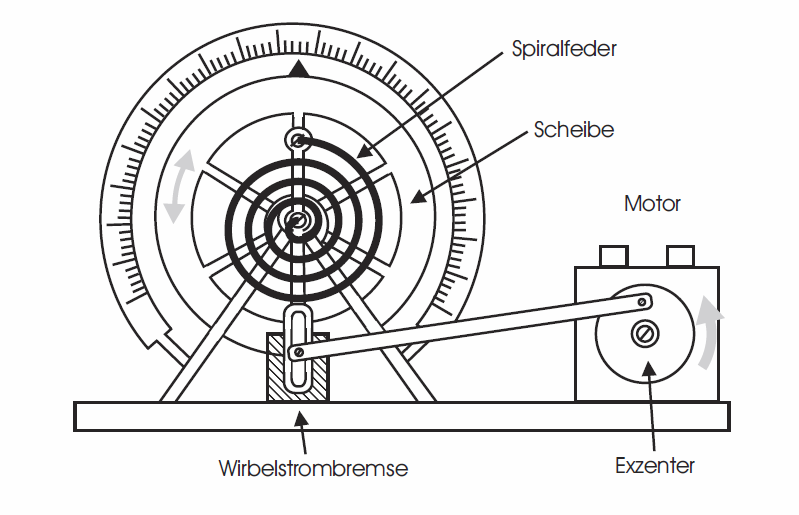
\includegraphics[width=\textwidth]{Drehpendel.png}
			\caption{Drehpendel nach Pohl}
			\label{abb:Drehpendel}
		\end{figure}
		
	\section{Messunsicherheiten der folgenden Versuche}
		
		\begin{itemize}
			\item Unsicherheit bei der Computermessung: 
			\begin{itemize}
				\item Zeitungenauigkeit: $u(t) = \frac{\SI{0,05}{\second}}{2\sqrt{3}}$
				
				Hierbei handelt es sich um die Breite der Abtastrate.
				
				\item Positionsunsicherheit: $u(x) = \frac{\SI{1}{mm}}{2\sqrt{3}}$
				
				Dies ist die Summe aller nicht einzeln bestimmbarer Unsicherheiten (Seildehnung, CASSY-Unsicherheit)			
			\end{itemize}
			\item Unsicherheit der Stoppuhr:
			$u_\text{Uhr}(t) = \sqrt{u_\text{Digital}(t)^2 + u_\text{Reaktion}(t)^2}$.
			Dabei ist $u_\text{Digital}(t) = \frac{\SI{10}{ms}}{2\sqrt{3}}$ und $u_\text{Reaktion}(t) = \frac{\SI{100}{ms}}{2\sqrt{6}}$ für die Reaktionszeit
			\item Unsicherheit des Multimeters: 
			$u_\text{Multi}(U) = \sqrt{u_\text{Digital}(U)^2 + u_\text{Prozent}(U)^2}$.
			Messreichweite von \SI{20}{V}.
			Mit $u_\text{Digital}(U) = \frac{\SI{0,01}{V}}{2\sqrt{3}}$ und $u_\text{Prozent}(U) = 0,005 \cdot U$  (0.5\% des angegebenen Wertes)
			\item Unsicherheit für die Stromquelle: 
			$u_\text{Strom}(I) = u_\text{Digital}(I) = \frac{\SI{0,01}{A}}{2\sqrt{3}}$
			\item Unsicherheit für die manuelle Ablesung der Auslenkung: 
			$a = \SI{2}{mm}$, da der Wert nicht immer leicht abzulesen war.		
			Es sei $u_\text{Analog}(x) = \frac{\SI{2}{mm}}{2\sqrt{6}}$.
		\end{itemize}
	
	\section{Versuch zu freien Schwingungen}
		
		Bei dem ersten Versuch befassen wir uns mit freien Schwingungen, welche wir mit dem Drehpendel nach Pol imitieren. Für diese Schwingung bestimmen wir anhand unserer Messungen die Eigenfrequenz bzw. die des Pendels.
		
		\subsection*{Methoden}
			
			Zur Bestimmung der Eigenfrequenz betrachten wir zunächst harmonische Schwingungen.					
			Für einen Drehschwinger mit Trägheitsmoment der Kreisscheibe $J$, rücktreibendem Drehmoment $-D\varphi$ (wobei $D$ Federkonstante) und bremsendem Drehmoment $-r\dot{\varphi}$, welches proportional zur Winkelgeschwindigkeit $\omega$ ist, lautet die Bewegungsgleichung der harmonischen Schwingung:
			\begin{align} 
				J\ddot{\varphi}+r\dot{\varphi}+D\varphi=0 \\
				\text{und in der Normalform: } \quad  \ddot{\varphi}+2\rho\dot{\varphi}+\omega_0^2\varphi=0 \label{eq:HarmonischeSchwingung}\\
				\text{wobei: } \quad  \omega_0^2 = \frac{D}{J} \text{und } 2\rho = \frac{r}{J}
			\end{align} 
			Da wir bei der freien Schwingung jedoch keine Dämpfung vorliegen haben, ist $2\rho = 0$ und $\omega_0$ somit unsere Eigenfrequenz.
			
			Wir bestimmen die Eigenfrequenz des Pendel in diesem Versuch einmal über die Messung, die der Computer durchführt und einmal indem wir die Zeit, welche das Pendel für zehn Schwingungen braucht, mit einer Stoppuhr messen.
		
		\subsection*{Messung}
			
			Nach 20 Messungen mit jeweils zehn Schwingungen erhalten wir einen Mittelwert für die Periodendauer von
			$\bar{T} = \SI{1,8332+-0,03863}{\second}$.		
			Und somit für die Frequenz $\omega=1/T = \SI{0,5454+-0,0114}{\per\second}$ mit der Unsicherheit $u(\omega) = \frac{u(T)}{T^2}$.
			
			Bei der Computermessung hingegen haben wir nur zehn mal zehn Schwingungen betrachtet, da der mit dem Messgerät verbundene Faden sich nach der zehnten Messung löste.
			Auch hier haben wir für die ersten zehn gemessenen Schwingungen die Periodendauer bestimmt (von erstem bis zum elften Minimum), um den erhaltenen Wert besser mit dem der Stoppuhr vergleichen zu können. 
			Dies lieferte uns einen Wert für die gemittelte Periodendauer: $\bar{T}=\SI{1,8255+-0,0020}{s}$.
			Wir haben diesen Wert erhalten, indem wir $dT = T_2 - T_1$ als zeitlichen Abstand zwischen dem ersten Minimum($T_1$) und dem Elften($T_2$) wählten. Für die Unsicherheiten nehmen wir an, dass
			$u(T_1) = u(T_2)$ gilt. Insgesamt ergab sich für die Unsicherheit der Periodendauer:
			\begin{align}
				u(dT) &= \sqrt{\left( \frac{\partial\,dT}{\partial\,T_1} \cdot u(T_1)\right)^2 +\left( \frac{\partial\,dT}{\partial\,T_2} \cdot u(T_2)\right)^2}\\
				&= \sqrt{(-u(T_1))^2 + (u(T_2))^2}\\
				&= \sqrt{2 u(T)^2} = \sqrt{2} u(T)
			\end{align}		
			Für die Frequenz $\omega$ ergibt sich damit dann: $\omega=\SI{0,5477+-0,0006}{\per\second}$.
					
		\subsection*{Schlussfolgerung}
			
			Wie im Methodenteil beschrieben können wir im Fall einer ungedämpften Schwingung davon ausgehen, dass die von uns gemessene Eigenfrequenz $\omega$ gerade der Frequenz $\omega_0$ des Systems ohne äußeren Einfluss entspricht. 
			
			Entsprechend den Erwartungen erhalten wir ähnliche Werte bei beiden Messungen für die Frequenz des Systems. Merklich ist, dass die Unsicherheit der Computermessung deutlich geringer als die der Messung von Hand ausfiel, was ebenfalls zu erwarten war.
				
	\section{Versuch zu gedämpften Schwingungen}
		
		In diesem Versuch betrachten wir gedämpfte Schwingungen, welche wie auch Ungedämpfte harmonisch sind.
		Zum Dämpfen des Pendels verwenden wir die Wirbelstrombremse welche an dem Pendel angebracht ist, wie oben beschrieben. 
				
		\subsection*{Methoden}
			
			Betrachten wir nun erneut \refeq{HarmonischeSchwingung}, wobei dieses mal $2\rho \neq 0$ ist, so
			erhalten wir mit dem Ansatz $\varphi (t)=C\cdot e^{\omega t}$ die Lösung: 
			\begin{equation}
				\omega_{1,2}= -\rho \pm \sqrt{\rho^2-\omega_0^2} \label{eq:HarmonischeFrequenz}
			\end{equation}
			An dieser Stelle müssen wir differenzieren, in welchem Verhältnis $\rho$ und $\omega_0$ stehen.
			Die beiden Fälle, bei denen reelle Werte aus dem Wurzelausdruck entstehen, den sogenannten Kriechfall (bei $\rho > \omega_0$) bzw. aperiodischen Grenzfall (bei $\rho = \omega_0 $), werden wir im Folgenden nicht genauer betrachten. 
			
			Für den Fall, dass $\rho < \omega_0 $ ist, erhalten wir eine mit $e^{\rho t}$ gedämpfte Kosinusschwingung mit der Frequenz $\omega = \sqrt{\omega_0^2-\rho^2}$, da wir nur den Realteil unserer Lösung betrachten. Wir messen die Eigenfrequenz $\omega$ und bestimmen die Dämpfung $\rho$, indem wir für $\omega_0$ die Frequenz des ersten Versuches nehmen. 
						
			Hier und in den folgenden Versuchen betrachten wir nur noch die von dem Computer aufgenommenen Messergebnisse. Wir messen hier die Zeit, bis das Pendel komplett aufhört zu schwingen zur Bestimmung der Eigenfrequenz und führen die Messung für verschiedene Dämpfungen $\rho$ durch. Um die Stärke der Dämpfung einzustellen verwenden wir verschiedene Eingabestromstärken für die Wirbelstrombremse.
		
		\subsection*{Messung}
		
			Für die folgenden Stromstärken haben wir die Frequenz $\omega$ gemessen. Das Umstellen von \refeq{HarmonischeFrequenz}, zur Berechnung der Dämpfung $\rho$, lieferte uns folgende Messergebnisse:	
			
			\begin{table}[ht]
				\centering
				\begin{tabular}{l|S|S|S}
					\hline
					{Stromstärke $I$} & {\SI{0.25}{\A}} & {\SI{0.5}{\A}} & {\SI{0.75}{\A}} \\
					\hline
					{Eigenfrequenz $\omega$} \quad
					& \SI{10000}{\s^{-1}}	%TODO
					& \SI{10000}{\s^{-1}}
					& \SI{10000}{\s^{-1}}\\
					\hline
					{Dämpfung $\rho$}
					& \SI{10000}{\s^{-1}}
					& \SI{10000}{\s^{-1}}
					& \SI{10000}{\s^{-1}} \\
					\hline
				\end{tabular}
				\caption{Messergebnisse zur gedämpften Schwingung}
				\label{tab:MessungGedämpft}
			\end{table}
			Hierbei sind $\omega$ und $\rho$ positiv gewählt, da die negativen Werte physikalisch nicht sinnvoll sind. Die gemessenen Kurven der Auslenkung gegenüber der Zeit sind in \ref{} dargestellt. Wir erkennen  - - - %TODO
					
		\subsection*{Schlussfolgerung}
			
			Da wir hier den leicht gedämpften Fall betrachten sieht die Lösung der Differentialgleichung wie folgt aus:
			\begin{equation}
				\varphi (t)=C\cdot e^{\rho t}\cdot \cos{(\sqrt{\omega_0^2-\rho^2}t)}
			\end{equation}
			Übertragen wir diese Bewegung nun auf die Ergebnisse unserer Messung, so erkennen wir, dass - - - %TODO
			
	\section{Versuch zu erzwungenen Schwingungen}
	
		Nun betrachten wir erzwungene Schwingungen, welche wir mit Hilfe eines Motors an unserem Pendel erzeugen.
			
		\subsection*{Methoden}
			
			Erneut betrachten wir \refeq{HarmonischeSchwingung}, jetzt steht auf der anderen Seite jedoch nicht null sondern:
			\begin{align}
				\ddot{\varphi}+2\rho\dot{\varphi}+\omega_0^2\varphi= \mu cos(\omega t) \label{eq:ErzwungeneSchwingung}\\
				\text{wobei } \mu = \frac{M_0}{J}
			\end{align}
			$M_0$ ist hierbei die Amplitude der äußeren Anregung und $J$ wie zuvor das Trägheitsmoment der Kreisscheibe. Die angeregte Schwingung hat zudem die Frequenz $\omega$.
			Es bildet sich eine Überlagerung des harmonischen Teils mit der angeregten Schwingung. Da der harmonische Teil jedoch abfällt, schwingt das System nach dem Abfallen bzw. nach dem sogenannten Einschwingvorgang genau so wie die Anregung.
			Eine mögliche Lösung von \refeq{ErzwungeneSchwingung} setzt sich wie folgt zusammen:
			\begin{align}
				\varphi = \varphi_0 \cos{(\omega t-\alpha)} \label{eq:ErzwungeneSchwingungLsg}\\
				\text{mit } \quad \varphi_0 = \frac{\mu}{\sqrt{(\omega^2-\omega_0^2)^2+4\rho^2\omega^2}} \label{eq:ErzwungeneSchwingungAmp}\\
			\end{align}
			Die erzwungene Schwingung ist somit eine mit der Frequenz $\omega$ schwingende Kosinusfunktion. Die Phase von $\varphi$ hängt der Phase der Anregung um $\alpha$ hinterher (vgl. \refeq{ErzwungeneSchwingung} und \refeq{ErzwungeneSchwingungLsg}) und die Amplitude $\varphi_0$ von $\varphi$ ist zeitlich konstant und hängt von der Dämpfung $\rho$ des Systems ab.
			
			Im Resonanzfall ist die Amplitude maximal. Betrachten wir hierzu \refeq{ErzwungeneSchwingungAmp}, so erhalten wir, dass die Resonanzfrequenz bei $\omega_\textsc{R} = \sqrt{\omega_0^2-2\rho^2}$ liegt.
			
			Um die Frequenz der Anregung zu bestimmen, erstellen wir eine Kalibrierkurve, messen also die Umlaufdauer $T$ der Anregung, für verschiedene Spannungen an dem Motor, mit einer Stoppuhr. Diese Spannungen messen wir an dem Ausgang des Motors mit einem Multimeter.
			Zusätzlich bestimmen wir die Resonanzfrequenz $\omega_\textsc{R}$ für drei verschiedene Dämpfungen, die ungleich null sind [um die Resonanzkatastrophe zu vermeiden (dass die Amplitude $\varphi_0$ gegen unendlich geht)].
				
			Zuletzt betrachten wir die Phasenverschiebung $\alpha$ zwischen Anregung und Pendel für verschiedene Dämpfungen und Frequenzen. Dies übertragen wir zusätzlich auf das Fadenpendel.
		
		\subsection*{Messung}
			
			Für unsere Anregungsfrequenz haben wir in Abhängigkeit der Spannung die in \ref{} dargestellte Kurve aufgenommen. Diese verläuft linear.
			
			Die Ermittlung der Resonanzfrequenz  $\omega_\textsc{R}$ geschah hier für drei unterschiedliche Dämpfungen. Dazu haben wir jeweils ca. 20 Amplituden für die verschiedenen Anregungsfrequenzen aufgezeichnet, welche in den Figuren \ref{}, \ref{} und \ref{} dargestellt sind. Daraus nähern wir die in \reftab{MessungErzwungen} dargestellten Resonanzfrequenzen und Dämpfungen (anhand der Amplitudenposition) für die verschiedenen Stromstärken bei der Wirbelstrombremse.
			\begin{table}[ht]
				\centering
				\begin{tabular}{l|S|S|S}
					\hline
					{Stromstärke $I$} & {\SI{0.7}{\A}} & {\SI{0.4}{\A}} & {\SI{0.25}{\A}} \\
					\hline
					{Resonanzfrequenz $\omega_\textsc{R}$} \quad
					& \SI{10000}{\s^{-1}}	%TODO
					& \SI{10000}{\s^{-1}}
					& \SI{10000}{\s^{-1}}\\
					\hline
					{Dämpfung $\rho$}
					& \SI{10000}{\s^{-1}}
					& \SI{10000}{\s^{-1}}
					& \SI{10000}{\s^{-1}} \\
					\hline
				\end{tabular}
				\caption{Messergebnisse zur erzwungenen Schwingung}
				\label{tab:MessungErzwungen}
			\end{table}
			
			Danach haben wir die Phasenverschiebung $\alpha$ zwischen Anregung und Drehpendel beobachtet. Für niedrige Anregungsfrequenzen war $\alpha \approx 0$. Beide Schwingungen verliefen demnach in gleicher Phase. Im Resonanzfall war zu erkennen, dass die Phase der Anregung stets der Phase des Pendels um $\pi\cdot\frac{1}{2}$ voraus, war also bereits wieder bei null, wenn das Pendel bei einem Maximum/Minimum war. Bei hohen Frequenzen lag der Phasenunterschied $\alpha = \pi$, da wenn das Pendel bei einem Maximum war, die Anregung gerade bei einem Minimum war und umgekehrt.
			
			Das Übertagen der Phasenverschiebung auf ein Fadenpendel lieferte die gleichen Beobachtungen wie bei dem Drehpendel. Die Anregung wurde hierbei an dem Aufhängepunkt des Pendels simuliert.   
			
		\subsection*{Schlussfolgerung}
			
			- - -
			%TODO
			% Schlussfolgerung
			
	\section{Versuch zu nichtlinearen Schwingungen}
	
		Der letzte Versuch behandelt nichtlineare Schwingungen. Auch diese stellen wir mit Hilfe des Drehpendels dar. Dazu bringen wir ein Gewicht an der Scheibe des Pendels an.
		
		\subsection*{Methoden}
				
			Die Resonanzfrequenzen nichtlinearer Schwingungen lassen sich nicht, wie bei den vorherigen Schwingungstypen berechnen, da diese sich auch bei gleichen Anfangsbedingungen nicht gleich verhalten.
			
			Wir können die Resonanzfrequenz jedoch annähernd messen, indem wir die Auslenkung des Pendels mit Anregung messen und dabei die Frequenz der erzwungenen Schwingung langsam ändern.
			Hier fangen wir bei niedrigen Frequenzen an, erhöhen diese und nahe der Maximalfrequenz verringern wir sie wieder, bis wir bei unserem Ausgangspunkt angelangt sind.
		
		\subsection*{Messung}
			
			Unsere Messung, wie sie in \ref{} dargestellt ist, zeigt dass sich die Resonanzfrequenz mit der Zeit ändert. Bei dem Erhöhen der Anregungsfrequenz haben wir die Resonanzfrequenz zunächst bei einer Ausgangsspannung von ca. \SI{8,2}{\V} gemessen. Nach dem Verringern der Anregungsfrequenz jedoch haben wir unsere Resonanzfrequenz bei ca. \SI{6,4}{\V} gefunden. Nahe den gemessenen Resonanzfrequenzen, fiel die Auslenkung stark ab.
			Nahe der Resonanzfrequenz konnten wir für sie stabilen Schwingungszustände zwei gemischte Frequenzen ermitteln. %TODO
			
		\subsection*{Schlussfolgerung}
			
			- - -
			%TODO
			% Schlussfolgerung

	\vspace{1cm}		
	\section*{Literatur}
		\begin{description}
			\item[\refabb{Drehpendel}] Das hier verwendete Bild stammt aus \glqq Drehpendel\_Pohl\_Einführung.pdf\grqq
		\end{description}
\end{document} 